% !TeX root = Seminararbeit.tex

\documentclass[%
12pt,                % Schriftgröße
paper=a4,            % Papiergröße
captions=tableabove, % Beschriftungen für Tabellen oberhalb
]{scrartcl}

% ----------------------------------------------------
% Essential packages
% ----------------------------------------------------
\usepackage[utf8]{inputenc}
\usepackage[T1]{fontenc}

% ----------------------------------------------------
% Packages for layout adjustments
% ----------------------------------------------------

% Adjust line spacing
\usepackage{setspace}

% Publication quality tables
\usepackage{booktabs}

% ----------------------------------------------------
% Fonts
% ----------------------------------------------------
\usepackage{lmodern}
\renewcommand{\seriesdefault}{m}\selectfont

\newcommand\roboto{\fontfamily{Roboto-LF}\selectfont}
\newcommand*\robotocondensed{\roboto\fontseries{c}\selectfont}

\setkomafont{subject}{\large\robotocondensed}
\addtokomafont{title}{\LARGE}
\addtokomafont{subtitle}{\Large}
\setkomafont{author}{\normalsize\robotocondensed}
\addtokomafont{publishers}{\normalsize\robotocondensed}

% ----------------------------------------------------
% Colors
% ----------------------------------------------------
\usepackage{graphicx}
\usepackage[svgnames]{xcolor}
\definecolor{darkgreen}{rgb}{0.23,0.46,0.23}
\definecolor{smdsblue}{RGB}{0,69,134}

% ----------------------------------------------------
% Internal commands
% ----------------------------------------------------

\usepackage{etoolbox}
\makeatletter
\newcommand{\seminartype}[2]{%
  \subject{%
    Seminar\\
    \textit{\GetTranslationWarn{seminar@#1}}\\
    #2
  }
}
\newcommand{\advisor}[1]{%
  \publishers{%
    \GetTranslation{advisor}: #1\\
    \GetTranslation{institute}}
}
\newcommand{\email}[1]{\gdef\@email{#1}}
\newcommand{\matrno}[1]{\gdef\@matrno{#1}}
\newcommand{\institute}[1]{\gdef\@institute{#1}}
\newcommand{\useAI}[1]{\def\AIUse{#1}}
\makeatother

% Sprachauswahl:
%  main=* setzt die Hauptsprache für das Dokument
%  - ngerman --> deutsch
%  - english --> englisch
\def\languages{main=german,english}
%\def\languages{main=english,ngerman}

% Art und Zeitpunkt des Seminars:
% - SEvS    Software Engineering für verteilte Systeme
% - ML     Machine Learning
% - SEisS    Software Engineering in sicherheitskritischen Systemen
\seminartype{SEvS}{Sommersemester 2024}

% Haupttitel der Arbeit
\title{Recent Approaches to accelerate CP Solving}
% Untertitel der Arbeit -- für Seminararbeiten nicht benötigt
% \subtitle{Concepts, Technologies, and Applications}

% Name, Matrikelnummer und E-Mail-Adresse
\author{---}
\matrno{---}
\email{---e}

% Transparenzangabe zur Verwendung
% künstlicher Intelligenz (KI)-basierter Tools. 
% Mögliche Optionen:

% - No          Keine KI-basierten Tools verwendet:
%               Sämtliche Inhalte sind eigenständig und ohne die
%               Unterstützung von Algorithmen oder Software, 
%               die auf KI basiert, entstanden.

% - Support     Verwendung KI-basierter Tools zur sprachlichen 
%               Verbesserung oder Korrektur des Textes:
%               Dies umfasst die Nutzung von Software zur 
%               Grammatikprüfung, Rechtschreibkorrektur 
%               und stilistischen Optimierung des Textes. 

% - Content     Verwendung KI-basierter Tools zur (teilweisen) 
%               Generierung von Inhalt:
%               Dies beinhaltet die Nutzung von KI für die Erstellung 
%               von Textabschnitten, Konzeptionierung von Ideen oder
%               Bereitstellung struktureller oder inhaltlicher Vorschläge.

\useAI{Content}

% Datum der Abgabe
\date{---}

\advisor{---}

%%% Local Variables:
%%% mode: latex
%%% TeX-master: "Seminararbeit"
%%% End:


% ----------------------------------------------------
% Multi-lingual documents with Babel
% ----------------------------------------------------
\usepackage{csquotes}
\usepackage[\languages]{babel}

% ----------------------------------------------------
% Hyperlinks in PDF documents
% ----------------------------------------------------
\usepackage[%
bookmarks=true,         %
bookmarksopenlevel=1,   %
bookmarksopen=true,     %
bookmarksnumbered=true, %
plainpages=false,       % correct hyperlinks
pdfpagelabels=true,     % view TeX pagenumber in PDF reader
colorlinks=true,        % color highlight links
allcolors=black,        % make all links black by default
urlcolor=smdsblue,      % URL color
]{hyperref}

\makeatletter
\AtEndPreamble{
  \hypersetup{
    pdftitle=\@title,
    pdfauthor=\@author
  }
}
\makeatother

% Provides a solution to the problem with hyperref that links
% to floats actually anchor to the place below the float's caption,
% instead of anchoring to the beginning of the float
\usepackage[all]{hypcap}

% ----------------------------------------------------
% Code listings
% ----------------------------------------------------
\usepackage{listings}
\lstset{%
  frame=single,                             % Add a single line frame around listings
  frameround=ftft,                          % Rounded frame corners on top left and bottom right
  backgroundcolor=\color{gray!5},           % Slight gray shade for listings
  rulecolor=\color{black!30},               % Gray frame outline
  xleftmargin=.125\textwidth,               % Extra left margin
  xrightmargin=.125\textwidth,              % Extra right margin
  basicstyle=\small\ttfamily,               % General font style for listings
  keywordstyle=\bfseries,                   % Font style for keywords
  commentstyle=\color{gray},                % Font style for comments
  stringstyle={},                           % Font style for string literals
  numbers=left,                             % Show line numbers
  stepnumber=1,                             % Step increments for line numbers
  numberstyle={\sffamily\tiny\color{gray}}, % Font style for line numbers
  numbersep=2em,                            % Space between line numbers and code
}

% ----------------------------------------------------
% Bibliography management
% ----------------------------------------------------
\usepackage[%
backend=biber,      % Use biber to process bibliographies
natbib=true,        % Provide natbib-compatible citation commands
sorting=none,       % Sort citations by occurrence in the document
style=numeric-comp, % Use compressed numeric citations, e.g. [1-3; 5]
block=space,        % Add a little spacing inside bibliography entries
]{biblatex}
\addbibresource{literature.bib}

% Use main body font for URLs in bibliography
\urlstyle{same}

% Suppress page numbering on table of contents page(s). Works at least on one-page TOC.
\AtBeginDocument{\addtocontents{toc}{\protect\thispagestyle{empty}}} 

% Intelligent cross-referencing
% Note: Must be loaded at end of preamble (esp. after hyperref)
\usepackage{cleveref}

% ----------------------------------------------------
% Localization / translations
% ----------------------------------------------------
\usepackage{translations}

% Translations for seminar names
\NewTranslation{ngerman}{seminar@SEvS}{Software Engineering für verteilte Systeme}
\NewTranslationFallback{seminar@SEvS}{Software Engineering for Distributed Systems}
\NewTranslation{ngerman}{seminar@MS}{Machine Learning}
\NewTranslationFallback{seminar@MS}{Machine Learning}
\NewTranslation{ngerman}{seminar@SEisS}{Software Engineering in sicherheitskritischen Systemen}
\NewTranslationFallback{seminar@SEisS}{Software Engineering in Safety- and Security-Critical Systems}

% Generic translation used in template
\NewTranslation{ngerman}{advisor}{Betreuer}
\NewTranslation{ngerman}{matrno}{Matrikelnummer}
\NewTranslation{ngerman}{institute}{Softwaremethodik für verteilte Systeme (Prof. Bauer)\\Universität Augsburg}
\NewTranslation{ngerman}{regularlit}{Literatur}
\NewTranslation{ngerman}{onlinelit}{Online-Quellen}
\NewTranslation{ngerman}{honesty@title}{Eidesstattliche Erklärung}
\NewTranslation{ngerman}{honesty@body}{%
  Ich versichere, dass ich die vorliegende Arbeit ohne fremde Hilfe und ohne Benutzung anderer
  als der angegebenen Quellen angefertigt habe, und dass die Arbeit in gleicher oder ähnlicher
  Form noch keiner anderen Prüfungsbehörde vorgelegen hat.\endgraf
  Alle Ausführungen der Arbeit, die wörtlich oder sinngemäß übernommen wurden, sind als solche
  gekennzeichnet.
}
\NewTranslation{ngerman}{aiused@no}{%
  Bei der Erstellung dieses Dokuments wurde keinerlei auf künstliche Intelligenz 
  (KI)-basierte Software verwendet.
}
\NewTranslation{ngerman}{aiused@support}{%
  Bei der Erstellung dieses Dokuments wurde künstliche Intelligenz (KI)-basierte 
  Software ausschließlich zur sprachlichen Verbesserung und Korrektur verwendet. 
}
\NewTranslation{ngerman}{aiused@content}{%
  Bei der Erstellung dieses Dokuments wurde künstliche Intelligenz (KI)-basierte 
  Software zur Generierung von Inhalten verwendet. 
}


% English fallback text
\NewTranslationFallback{advisor}{Advisor}
\NewTranslationFallback{matrno}{Matriculation number}
\NewTranslationFallback{institute}{Software Methodologies for Distributed Systems (Prof. Bauer)\\University of Augsburg}
\NewTranslationFallback{regularlit}{Literature}
\NewTranslationFallback{onlinelit}{Online resources}
\NewTranslationFallback{honesty@title}{Declaration of Academic Honesty}
\NewTranslationFallback{honesty@body}{%
  Hereby, I declare that I have composed the presented paper independently on my own and without
  any other resources than the ones indicated. All thoughts taken directly or indirectly from external
  sources are properly denoted as such.\endgraf
  This paper has neither been previously submitted to another authority nor has it been published yet.
}
\NewTranslationFallback{aiused@no}{%
  No artificial intelligence (AI)-based software was used in the creation of this document.
}
\NewTranslationFallback{aiused@content}{%
  Artificial intelligence (AI)-based software was used for content generation in the 
  creation of this document.
}
\NewTranslationFallback{aiused@support}{%
Artificial intelligence (AI)-based software was used exclusively for linguistic improvement 
and correction in the creation of this document.
}


%%% Local Variables:
%%% mode: latex
%%% TeX-master: "Seminararbeit"
%%% End:


\begin{document}
\pagenumbering{roman}	
% !TeX root = Seminararbeit.tex

\begin{titlepage}
  \onehalfspacing
  \makeatletter
  \vspace*{1em}
  \begin{center}
    \ifdefempty{\@subject}{}{%
      {\usekomafont{subject}\@subject}
      \par\vspace{2em}
    }
    {\usekomafont{title}\@title}
    \ifdefempty{\@subtitle}{}{%
      \par\vspace{.5em}
      {\usekomafont{subtitle}\@subtitle}
    }
    \par\vspace{2em}
    \singlespacing
    {\usekomafont{author}%
      \@author\par
      \GetTranslation{matrno}: \@matrno\par}
    \texttt{\@email}
    \par\vspace{1.5em}
    {\usekomafont{publishers}\@publishers}
  \end{center}
  \makeatother

  \begin{abstract}
    \noindent%
    \paragraph*{\abstractname}
    \textcolor{red}{Bitte Dateien \texttt{settings.tex} und \texttt{titlepage.tex} anpassen.}
    
    Abstract Lorem ipsum dolor sit amet, consectetuer adipiscing elit, sed diam nonummy nibh euismod tincidunt ut laoreet dolore magna aliquam erat volutpat. Ut wisi enim ad minim veniam, quis nostrud exerci tation ullamcorper suscipit lobortis nisl ut aliquip ex ea commodo consequat.
  \end{abstract}

  \vfill
  \centering
  
\includegraphics[height=38mm]{figures/uni_siegel}
\end{titlepage}
%%% Local Variables:
%%% mode: latex
%%% TeX-master: "Seminararbeit"
%%% End:


\tableofcontents

\clearpage
\pagenumbering{arabic}


\section{Einleitung: Verwendung von Constraint Programming}
\label{sec:Einleitung-Verwendung-von-Constraint-Programming}
Constraint Programming (CP) spielt in einem weiten Bereichen heutiger modernen
Anwendungen eine große Rolle in welchen Optimierungsproblemen mit
Nebenbedingungen gelöst werden müssen. Anwenungen hierzu sind unter anderem:
Vehicel Routing, Scheduling, Planung, Konfiguration, Ressourcenallokation und
Kombinatorische Optimierung. Auch findet jährlich die  Conference on Principles
and Practice of Constraint Programming statt, in welcher aktuelle
Forschungsergebnisse im Bereich CP diskutiert werden, wodurch die Wichtigkeit
des Themenfeldes unterstrichen wird. \cite{CP20we}. Neben dem Klassischen
Problem der Kursplannung \cite{duboi96jo} in der immer schneller werden Zeit,
gib es auch in der Industrie eine Vielzahl von Scheduling Problemen, wie der
Zuweiung von Aufträgen zu Maschinen \cite{gedik16jo}. Auch wurden CP Ansätze für
die Konfiguration von Netzwerken verwendet \cite{ardisjo}. Ein weit Verbreitetes
Kombinatirsches Optimierungsproblem ist das 3-SAT Problem. Es beschreibt die
Frage ob eine Formel in konjunktiver Normalform (KNF) mit Klauseln aus jeweil 3
Literalen erfüllbar ist.
\cite[271]{rossi06bo} 
Beispielsweise löst

$$x_1=\mathrm{false},x_2=\mathrm{false},x_3=\mathrm{false},x_4=\mathrm{false}$$

das folgende 3-SAT Problem:

$$(\lnot x_1\lor x_2\lor x_3)\land(x_1\lor\lnot x_2\lor x_4)\land(x_2\lor
x_3\lor\lnot x_4)$$

Besonders Vehicel Routing ist in der heutighen Zeit für viele Unternehmen in der
Logistikbranche und dem Flexiblen Transport von großer Bedeutung.
\cite[1]{delec22jo}. Je nach Anwendungen und Problemstellung können
unterschiedliche Constraint Programming Ansätze verwendet werden. Es exisiteren
diveres Toolboxen um Contraint Programming Problem zu Lösen. Für das Vehicel
Routing Problem, welches das Problem beschreibt für n Fahrzeuge und m Orte den
kürzesten gesamt Weg zu finden \cite[222]{labor18jo}, kann beispielseise der IBM
ILOG CP Optimzer verwendet werden.\cite{IBMIwe} Je nach Problemstellung gibe es
eine Viehlzahl von weitern Toolboxen \cite{Solviwea}, Or-tools von Google ist
eine weitere zum lösen von Constraint Programming (CP), Linear Programming (LP),
Integer Programming (IP) und Boolean Satisfiability (SAT) Problemen.
\cite{ORToowe}, Geocode ist eine Open Source Variante basierend auf C++
\cite{GECODwe} und Chuffed is eine Varainte welche "lazy clause generation"
ausnutzt um CP Probleme schneller zu lösen \cite{Chuff24co}. MiniZinc vereint
unter anderem die im Vorherigen beschriebenen Softwarebibliotheken zu einer
Ausdrucksspache zum Lösen von einer Vielzahl von LP, Transportprobleme (TP) und
SAT Problemen. \cite{MiniZwe}. Unter dem selben Namen wird Jährlich die MiniZinc
Challenge ausgetragen, in der ein Parkour von Constraint Modelen gelöst werden
muss. Am Ende werden die Solver nach Anzahl der gelösten Modelle, der Zeit und
der Qualität der Lösung bewertet. \cite{Homewe}. Gerade bei großen
Problemstellungen oder wenn beispielweise in der Forschung oft üblich, mehrere
Lösung oder Besondere Ansprüche an die Qualität und Genauigkeit der Lösung
gestellt werden kann die Ausführung oft lange dauern, weshalb die benötigte Zeit
der Solver von großer Bedeutung ist. Die folgende Arbeit soll hierzu aktuelle
Ansätze vorstellen mit denen CP Problme schneller gelöst werden können. 

%\cite{keylist}

\section{Grundlagen}
\label{sec:Grundlagen}
Grundlegend gibt es zwei Arten von Constraint Problemen, Constraint Satisfaction
Probleme (CSP) und Constraint Optimization Problem (COP). Ein CSP beschreibt im
wesentlichen ein Problem, bei dem Nebenbedingungen festlegen welche Werte die
Variablen annehmen können. \cite[13]{rossi06bo} Ziel hierbei kann es entweder
sein zu überprüfen ob eine Lösung existiert, eine mögliche Lösung zu finden oder
die Menge aller möglichen Lösungen zu bestimmen. Ein COP ist eine Erweiterung
des CSP, bei dem zusätzlich eine Zielfunktion minimiert werden müssen.
\cite[171]{rossi06bo}. Ebeso kann es hierbei auch darum gehen zu überprüfen ob
das Problem überhaupt lösbar ist, eine mögliche Lösung zu finden oder die
optimale Lösung zu finden.


\subsection{Constraint Satisfaction Probleme}
\label{sec: Constraint Satisfaction Probleme}
Ein CSP lässt sich durch ein Tripel $P=(X,D,C)$ beschreiben, wobei $X=\langle
x_{1},x_{2},\ldots,x_{n}\rangle$  ein n-Tupel von Variablen, $D=\langle
D_{1},D_{2},\ldots,D_{n}\rangle$ ein n-Tupel von Domänen, so dass , so dass
$x_i\in D_{i}$ erfüllt ist und $C=\langle C_1,C_2,\ldots,C_t\rangle$ eine Menge
von Bedingungen beschreibt. Jede Bedindingung $C_j$ ist hierbei eine Untermenge
des Cartesischen Produkts über $D$. Eine Lösung für ein CSP ist ein n-Tupel
$A=\langle a_1,a_2,\ldots,a_n\rangle $ so dass $a_i\in D_i$ für alle $i$ und $A
\in C_j \quad \forall j$ \todo{revisit Formula}. \cite[16]{rossi06bo} Ein
Beispiel für ein CSP ist das oben beschriebene 3-SAT Problem. Das lösen eines
3-SAT Problems ist NP-Vollständig, was bedeutet das es keine effiziente
Algorithmus gibt, der das Problem in Polynomialzeit lösen kann.
\cite[17]{rossi06bo}. Eine einfache Möglichkeint ein CSP zu lösen ist die
Verwendung von Backtracking. Hierbei wird eine Variable nach der anderen belegt
und bei einem Widerspruch wird ein Schritt zurückgegangen und eine andere
Variable belegt. \cite[21]{rossi06bo} Interessant ist auch, dass  sich auch alle
k>3-SAT Probleme auf ein 3-SAT Problem reduzieren lassen wodurch auch das k>3
SAT Problem NP-Vollständig ist. \cite[206]{gritz13bo} Snd die Domänen der
Variablen auf boolesche Werte beschränkt handelt es sich um ein Boolean
Satisfiability  Problem (SAT).


\subsection{Constraint Optimization Problem}
\label{sec: Constraint Optimization Problem}
Viele Probleme in der echten Welt Welt suchen nicht nur eine Lösung, sondern die
optimale Lösung. Solche Probleme lassen sich durch ein Constraint Optimization
Problem modellieren. Hierzu wird die Problemstellung um eine Zielfunktion
erweitert die minimiert oder maximiert werden soll. Ein COP lässt sich durch ein
Tripel $P=(X,D,C,f)$ beschreiben, wobei die ersten drei Elemente wie bei einem
CSP sind und $f$ eine Zielfunktion ist. \cite[22]{amadi15jo}. In der Physik oder
den Ingenieurwissenschaften ist werden COP auch oft in Funktionsdarstellung
beschrieben.
\begin{align*}
    &\text{minimize:} \quad f(x) \\
    &\text{subject to:} \\
    &\quad g_j(x) \leq 0 \\
    &\quad h_l(x) = 0 \\
    &\quad \underline{x_i} \leq x_i \leq \overline{x_i}
\end{align*}
Hierbei beschreibt $g_j(x)$ und $h_l(x)$ die Nebenbedingungen $C$, wobei
ersteres eine Ungleichungsrestriktionen und letzteres eine Gleichungsrestriktion
darstellt. Die letzte Gleichung beschreibt die Domäne $D$ der Variablen.
\cite[154]{marti21bo}. Je nach Art der Probemstellung unterscheiden sich die
verwendeten Algorithmen. Sind beispielseise die Nebenbedingungen und die
Zielfunktion linear handelt es sich um ein Linear Programming Problem (LP).
Dieses lässt sich beispielseise mit dem Simplex Algorithmus lösen. Das Verfahren
beruht darauf dass die Nebenbedingungen einen n-dimensionalen Polyeder
aufspannen und die optimale Lösung auf einer Ecken des Polyeders liegt. Der
Simplex Algorithmus sucht nun nun nacheinander die Ecken ab bis die optimale
Lösung gefunden wurde. Beschränkt man sich bei den Lösungen auf ganzzahlige
Werte Spricht man von einem Integer Programming Problem (IP). Diese lassen sich 
mit dem Branch-and-Bound Algorithmus lösen. \cite{dakin65jo}
\cite[99]{hofst07bo}
\begin{figure}[h]
    \centering
    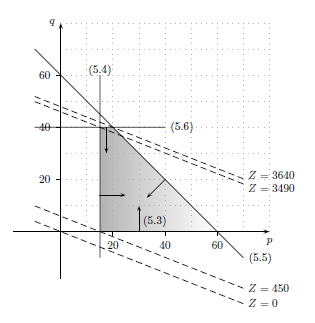
\includegraphics[width=0.5\textwidth]{figures/Simplex.PNG}
    \caption{Polyeder beschreibt Nebenbedingungen, Gestrichelte Linie die
    Zielfunktion,  Ecken sind mögliche Lösungen \cite[100]{hofst07bo}}
    \label{fig:bild}
\end{figure}
Oft lassen sich Probleme jedoch nur über nichtlineare Zusammenhänge beschreiben.
Eine Möglichkeit solche Probleme zu lösen ist die Verwendung von
Gradientenverfahren. \cite[153]{marti21bo}. Ein Problem bei der Verwendung von
diesen ist jedoch, dass sie je nach Initialisierung oft nur lokale Minima
finden. \cite[9]{boyd04bo}. Ein Ansatz um dieses Problem zu umgehen ist die
Verwendung von konvexen Funktionen. Dabei wird die nichtlineare Funktion durch
eine konkave Zielfunktion approximiert. \cite[11]{boyd04bo} Dies ist von
Vorteil, da konvexe Funktionen nur ein lokales Minimum haben.
\cite[7]{noced06bo}. Durch die einfachere Lösbarkeit von konvexen
optimierungsproblemen, spielen Sie auch in der Literatur eine wichtig Rolle.
\cite[8]{boyd04bo}. 



\section{Recent Approaches To Accelerate Constraint programms}
\label{sec:Recent Approaches To Accelerate Constraint programms}


\subsection{CP and Machine Learning}
\label{sec:CP and Machine Learning}

  
\subsection{Portfolio}
\label{sec:Portfolio}

  
\subsection{Model Based Optization}
\label{sec:Model Based Optization}

  
\subsection{Qunatum Acceleratedt}
\label{sec:Qunatum Accelerated}

  
\subsection{Combine CP and SAT}
\label{sec:Combine CP and SAT}

  
\subsection{Decompostion methods}
\label{sec:Decompostion methods}

  
\subsection{Search Heuristics}
\label{sec:Search Heuristics}


\section{Evaluation Performance Increase}
\label{sec:Evaluation Performance Increase}


% Literaturverzeichnis
\printbibliography[heading=bibintoc]

% Anhang
\include{appendix}

% Eidesstattliche Erklärung
% !TEX root = Seminararbeit.tex

\clearpage
\section*{\GetTranslation{honesty@title}}
\GetTranslation{honesty@body}

\vspace{2em}

\ifdefined\AIUse
    \expandafter\ifstrequal\expandafter{\AIUse}{No}{%
        \GetTranslation{aiused@no}
    }{%
        \expandafter\ifstrequal\expandafter{\AIUse}{Content}{%
            \GetTranslation{aiused@content}
        }{%
            \expandafter\ifstrequal\expandafter{\AIUse}{Support}{%
                \GetTranslation{aiused@support}
            }{% Fallback for undefined values
                \GetTranslation{aiused@no}
            }%
        }%
    }%
\else
    % Fallback, falls \useAI{} nie aufgerufen wurde
    \GetTranslation{aiused@no}
\fi

\vspace{2em}
\makeatletter
Augsburg, \@date
\par\vspace{1.5cm}
(\@author)
\makeatother

%%% Local Variables:
%%% mode: latex
%%% TeX-master: "Seminararbeit"
%%% End:


\end{document}